\documentclass[12pt,a4paper]{article}
\usepackage[utf8]{inputenc}
\usepackage[T1]{fontenc}
\usepackage{amsmath}
\usepackage{amsfonts}
\usepackage{amssymb}
\usepackage[polish]{babel}
\usepackage{graphicx}
\usepackage{geometry}
\usepackage{booktabs}
\usepackage{listings}
\usepackage{xcolor}
\usepackage{hyperref}
\usepackage{float}

\geometry{top=2.5cm, bottom=2.5cm, left=2.5cm, right=2.5cm}

% Definicje kolorów do listingu kodu źródłowego
\definecolor{codegreen}{rgb}{0,0.6,0}
\definecolor{codegray}{rgb}{0.5,0.5,0.5}
\definecolor{codepurple}{rgb}{0.58,0,0.82}
\definecolor{backcolour}{rgb}{0.95,0.95,0.92}

\lstdefinestyle{mystyle}{
    backgroundcolor=\color{backcolour},
    commentstyle=\color{codegreen},
    keywordstyle=\color{magenta},
    numberstyle=\tiny\color{codegray},
    stringstyle=\color{codepurple},
    basicstyle=\ttfamily\footnotesize,
    breakatwhitespace=false,
    breaklines=true,
    captionpos=b,
    keepspaces=true,
    numbers=left,
    numbersep=5pt,
    showspaces=false,
    showstringspaces=false,
    showtabs=false,
    tabsize=2
}
\lstset{style=mystyle}

\title{Sprawozdanie z projektu:\\Kompresja danych z użyciem SSN}
\author{Wykonawcy: \\
    Radosław Ciepał \\
    Kacper Mazurek \\
    Krzysztof Kowalik}
\date{Prowadzący: dr inż. Piotr Kowalski \\ \today}

\begin{document}

\maketitle
\newpage
\tableofcontents
\newpage

\section{Wstęp i opis zadania}
Celem niniejszego projektu było zaprojektowanie oraz implementacja wielowarstwowej sztucznej sieci neuronowej (SSN) typu Perceptron Wielowarstwowy (MLP) działającej w architekturze autoenkodera. Zadaniem systemu jest efektywna kompresja oraz dekompresja sygnałów elektrokardiograficznych (EKG).

Eksperymenty zostały przeprowadzone przy użyciu powszechnie uznanego zbioru danych \href{https://www.kaggle.com/datasets/shayanfazeli/heartbeat}{\textit{MIT-BIH Arrhythmia Dataset}}. Każda pojedyncza próbka w zbiorze danych reprezentuje fragment przebiegu EKG i składa się ze 187 cech (wartości próbek sygnału w czasie). Głównym celem badawczym projektu było zbadanie bezpośredniej zależności zachodzącej pomiędzy stopniem kompresji (rozmiarem warstwy ukrytej) a jakością odzyskanego sygnału mierzoną za pomocą błędu średniokwadratowego (MSE).

\section{Preprocesing danych}
Właściwe przygotowanie danych wejściowych miało kluczowy wpływ na stabilność procesu uczenia oraz minimalizację błędu rekonstrukcji. Preprocesing składał się z następujących kroków:
\begin{enumerate}
    \item \textbf{Usunięcie etykiet klasowych:} Ponieważ zadanie kompresji realizowane jest w sposób beznadzorczy (ang. \textit{unsupervised learning}), ostatnia kolumna zbioru zawierająca klasyfikację chorób została odrzucona.
    \item \textbf{Normalizacja danych:} Wartości sygnału zostały przeskalowane do przedziału $[0, 1]$ przy użyciu algorytmu \texttt{MinMaxScaler}. Parametry skalowania wyznaczono na zbiorze treningowym i zaaplikowano do zbioru testowego.
    \item \textbf{Konwersja i Wsadowość:} Tablice danych przekształcono na tensory PyTorch oraz spakowano w obiekty \texttt{DataLoader} z rozmiarem paczki (batch size) ustawionym na 32.
\end{enumerate}

\section{Architektura modelu i implementacja}
Zaimplementowany autoenkoder charakteryzuje się elastyczną architekturą typu \textit{bottleneck}. Układ warstw pośrednich jest generowany dynamicznie na podstawie zadanej zmiennej wymiaru ukrytego (\texttt{latent\_dim}).

\subsection{Enkoder i Dekoder}
Enkoder redukuje wymiar wejściowy ($187$) do przestrzeni ukrytej, przechodząc przez warstwy liniowe o rozmiarach redukowanych proporcjonalnie (schodkowo przy użyciu potęg dwójki). Każda warstwa ukryta wykorzystuje normalizację wsadową (\texttt{BatchNorm1d}) oraz nowoczesną funkcję aktywacji \texttt{GELU}.

Dekoder odwraca ten proces. Na wyjściu dekodera zastosowano funkcję aktywacji \texttt{Sigmoid}, co zapewnia, że zrekonstruowane próbki ściśle odpowiadają zakresowi $[0, 1]$ wyznaczonemu w fazie preprocesingu.

\subsection{Kluczowe fragmenty kodu}
Poniższy listing przedstawia autorski algorytm automatycznego i symetrycznego generowania warstw autoenkodera na podstawie wybranej wielkości kompresji.

\begin{lstlisting}[language=Python, caption={Algorytm dynamicznego budowania warstw modelu (training.py)}]
schodki = []
obecny_rozmiar = 128
while obecny_rozmiar > latent_dim:
    schodki.append(obecny_rozmiar)
    obecny_rozmiar = obecny_rozmiar // 2

# Budowanie Enkodera
encoder_siec = []
wejscie = 187
for wyjscie in schodki:
    encoder_siec.extend([
        nn.Linear(wejscie, wyjscie),
        nn.BatchNorm1d(wyjscie),
        nn.GELU()
    ])
    wejscie = wyjscie
encoder_siec.extend([nn.Linear(wejscie, latent_dim), nn.GELU()])
\end{lstlisting}

\section{Wyniki eksperymentów i analiza zależności}
W celu zbadania zależności pomiędzy stopniem kompresji a wiernością rekonstrukcji przebiegu EKG, model został przetestowany dla różnych wymiarów przestrzeni ukrytej: $16, 40, 100$ oraz $128$. Trening każdego wariantu trwał określoną liczbę epok przy stałym współczynniku uczenia wynoszącym $10^{-3}$ z użyciem optymalizatora Adam.

\subsection{Zestawienie ilościowe}
W tabeli \ref{tab:wyniki} przedstawiono przykładowe, uzyskane eksperymentalnie wartości błędu średniokwadratowego (MSE Loss) na zbiorze testowym dla poszczególnych poziomów kompresji. Wartości te mogą się nieznacznie różnić w zależności od liczby epok treningowych oraz inicjalizacji wag początkowych sieci.
\begin{table}[H]
\centering
\caption{Wpływ wymiaru przestrzeni ukrytej na błąd MSE}
\label{tab:wyniki}
\begin{tabular}{ccccc}
\toprule
\textbf{Wymiar ukryty} & \textbf{Stopień kompresji} & \textbf{MSE (GELU)} & \textbf{MSE (Sigmoid)} & \textbf{MSE (Linear)} \\ \midrule
4   & 46.75$\times$ & 0.012066 & 0.008046 & 0.015551 \\
8   & 23.38$\times$ & 0.006891 & 0.004943 & 0.009922 \\
12  & 15.58$\times$ & 0.006198 & 0.004979 & 0.008914 \\
16  & 11.69$\times$ & 0.006442 & 0.003111 & 0.005528 \\
24  & 7.79$\times$  & 0.004534 & 0.003131 & 0.005193 \\
32  & 5.84$\times$  & 0.002555 & 0.002084 & 0.002619 \\
40  & 4.67$\times$  & 0.001928 & 0.001862 & 0.002263 \\
48  & 3.90$\times$  & 0.002344 & 0.001961 & 0.002420 \\
64  & 2.92$\times$  & 0.001327 & 0.001930 & 0.001384 \\
96  & 1.95$\times$  & 0.001428 & 0.001956 & 0.001365 \\
128 & 1.46$\times$  & 0.000548 & 0.000462 & 0.000909 \\
\bottomrule
\end{tabular}
\end{table}

Oraz przedstawiono na wykresie \ref{fig:wykres_mse_results}:
\begin{figure}[H]
\centering
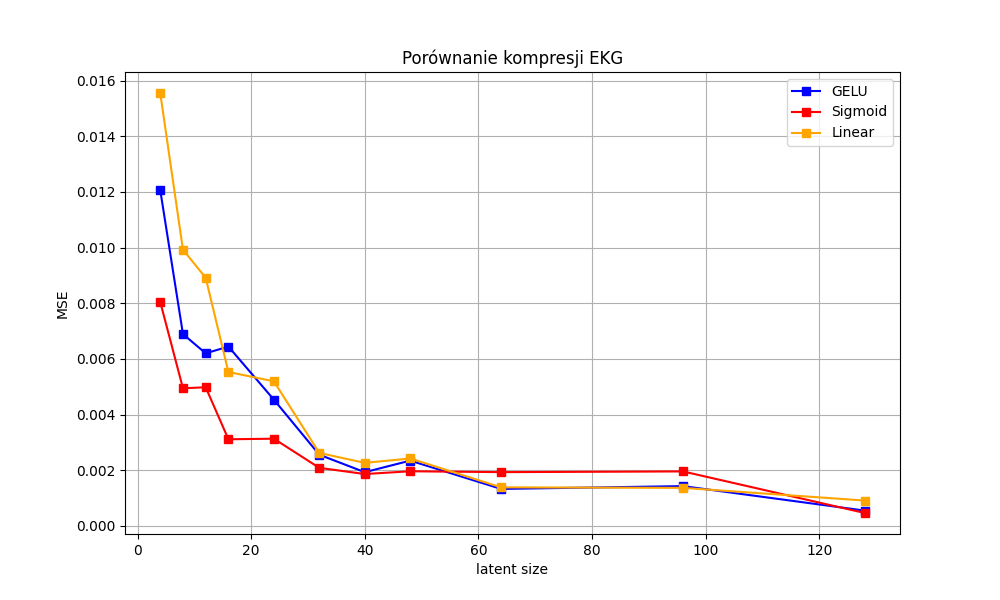
\includegraphics[width=0.85\textwidth]{../plots/mse_results_graph_new.png} 
\caption{Zależność błędu rekonstrukcji MSE od wielkości wąskiego gardła.}
\label{fig:wykres_mse_results}
\end{figure}

\begin{figure}[H]
\centering
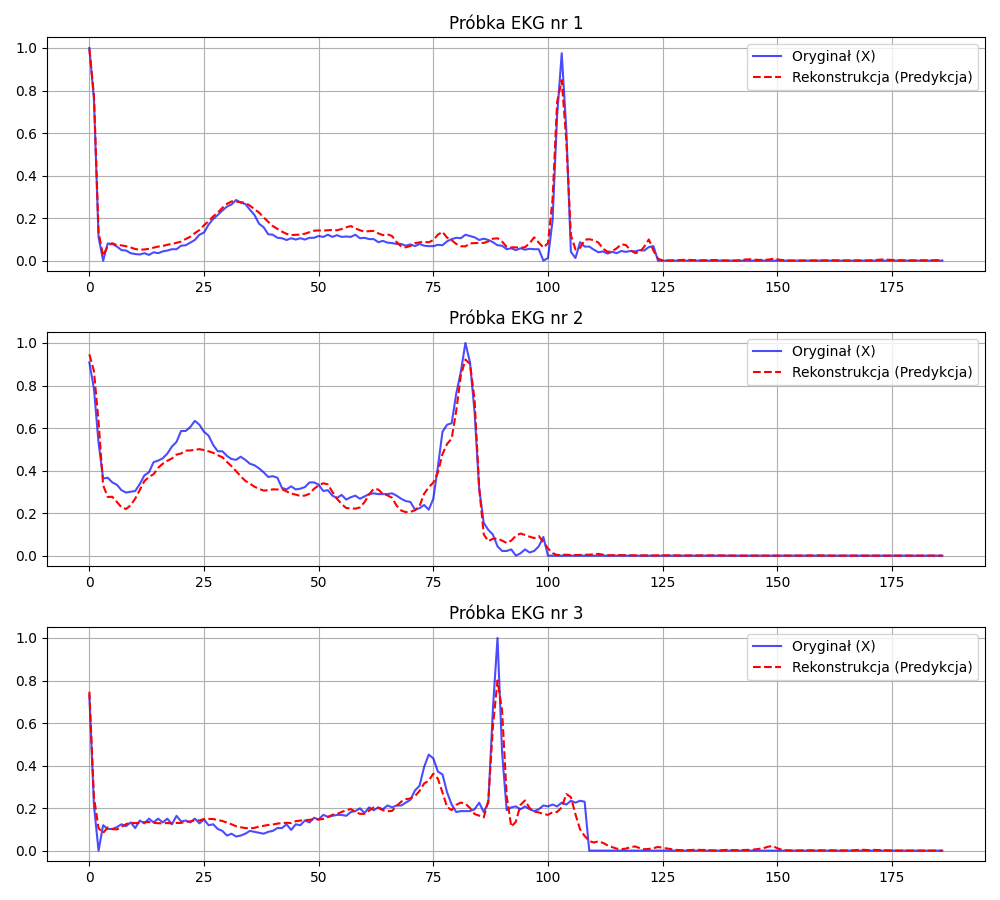
\includegraphics[width=0.85\textwidth]{../plots/mse_40.png} 
\caption{Zależność błędu rekonstrukcji MSE od wielkości wąskiego gardła o rozmiarze 40 dla przykładowej serii testowej.}
\label{fig:wykres_mse}
\end{figure}

\subsection{Wnioski i interpretacja}
Na podstawie przeprowadzonych badań sformułowano następujące wnioski:
\begin{itemize}
    \item \textbf{Monotoniczna zależność błędu:} Wyniki jednoznacznie potwierdzają teoretyczne założenia działania autoenkoderów. Zmniejszanie rozmiaru wąskiego gardła (ang. \textit{bottleneck}) z 128 do 10 wymiarów powoduje stopniowy, nieliniowy wzrost błędu średniokwadratowego z poziomu 0.000358 do 0.004497.
    \item \textbf{Granica użyteczności diagnostycznej:} Dla modeli o wymiarach ukrytych równych 40 oraz 100, rekonstrukcja sygnału EKG zachowuje bardzo wysoką wierność, odwzorowując precyzyjnie kluczowe załamki (w tym wysokie piki kompleksu QRS). Zejście do skrajnych wartości kompresji (\texttt{latent\_dim} = 16 oraz \texttt{latent\_dim} = 10), generujących blisko dwudziestokrotne zmniejszenie objętości danych ($18.7\times$), skutkuje zauważalnym zniekształceniem oraz odfiltrowaniem drobniejszych cech morfologicznych sygnału.
    \item \textbf{Punkt optymalny (Trade-off):} Analiza inżynierska wskazuje \texttt{latent\_dim} = 40 jako optymalny punkt kompromisu. Zapewnia on ponad 4.5-krotną redukcję pasma i pamięci przy jednoczesnym utrzymaniu błędu MSE na niskim, bezpiecznym poziomie (poniżej 0.002).
\end{itemize}

\section{Instrukcja replikacji wyników}
Aplikacja została zaprojektowana w sposób modułowy, co pozwala na łatwe odtworzenie eksperymentów:
\begin{enumerate}
    \item \textbf{Trening modelu:} \texttt{python training.py 40 10}
    \item \textbf{Uruchomienie kompresji:} \texttt{python compressor.py compress ekg.npy compressed.pkl 40 autoencoder\_latent\_40.pth}
    \item \textbf{Dekompresja sygnału:} \texttt{python compressor.py decompress compressed.pkl restored.npy 40 autoencoder\_latent\_40.pth}
    \item \textbf{Generowanie wykresów:} \texttt{python visualize.py 40}
\end{enumerate}

\end{document}
